% !TeX spellcheck = en_GB
%
\documentclass[presentation]{beamer}
\mode<presentation>{\usetheme{AMSCesenaPurpleAndGold}}
\setbeamertemplate{bibliography item}{\insertbiblabel}
\setbeamersize{description width=0.57cm}
%%%%%%%%%%%%%%%%%%%%%%%%%%%%%%%%%%%%%%%%%%%%%%%%%%%%%%%%%%%%%%%%%%%%%%%%%%%%%%%%
\usepackage{2p-kt-talk}
%%%%%%%%%%%%%%%%%%%%%%%%%%%%%%%%%%%%%%%%%%%%%%%%%%%%%%%%%%%%%%%%%%%%%%%%%%%%%%%%
\title[\twopkt]{
    \twopkt{}: A Kotlin Multi-Platform ecosystem for Symbolic AI 
}
%
% \subtitle{Extended Abstract}
%
% same authors order of the presented paper
\author[Ciatto G.]{
    \emph{Giovanni Ciatto}$^{*}$ % empth the presenting author
}
%
\institute[UniBo]{
    $^{*}$Dipartimento di Informatica -- Scienza e Ingegneria (DISI)
    \\
    \textsc{Alma Mater Studiorum} -- Università di Bologna
    \\
    \texttt{
        giovanni.ciatto@unibo.it % emph the presenting author's email
    }
}
%
\date[A.Y. 20-21]{
    Autonomous Systems Course, A.Y. 2020-2021
}
%%%%%%%%%%%%%%%%%%%%%%%%%%%%%%%%%%%%%%%%%%%%%%%%%%%%%%%%%%%%%%%%%%%%%%%%%%%%%%%%
\AtBeginSection[]{
    \begin{frame}<beamer>[shrink,noframenumbering]\frametitle{Next in Line\ldots}
        \mbox{~}
        \tableofcontents[sectionstyle=show/shaded,subsectionstyle=hide,subsubsectionstyle=hide]
        \mbox{~}
    \end{frame}
}
\AtBeginSubsection[]{
    \begin{frame}<beamer>[shrink,noframenumbering]\frametitle{Focus on\ldots}
        \mbox{~}
        \tableofcontents[sectionstyle=show/shaded,subsectionstyle=show/shaded,subsubsectionstyle=hide]%[currentsection,currentsubsection,sectionstyle=shaded,subsectionstyle=shaded,subsubsectionstyle=hide]
        \mbox{~}
    \end{frame}
}
%%%%%%%%%%%%%%%%%%%%%%%%%%%%%%%%%%%%%%%%%%%%%%%%%%%%%%%%%%%%%%%%%%%%%%%%%%%%%%%%
\begin{document}
%%%%%%%%%%%%%%%%%%%%%%%%%%%%%%%%%%%%%%%%%%%%%%%%%%%%%%%%%%%%%%%%%%%%%%%%%%%%%%%%

%\\\\\\\\\\\\\\\\\\\\\
\frame{\titlepage}
%\\\\\\\\\\\\\\\\\\\\\

\begin{frame}<beamer>[shrink,noframenumbering]\frametitle{Outline}
    \mbox{~}
    \tableofcontents
    \mbox{~}
\end{frame}

\section{Historical Perspective}

\subsection{Prolog History}

\begin{frame}{Implementations of Prolog -- Chronological Perspective}
    % !TEX root = 2p-kt-talk.tex
\begin{figure}[h]\centering
    \tiny
    \catcode`\@=11
    \def\chron@selectmonth#1{\ifcase#1\or January\or February\or
    March\or April\or May\or June\or
    July\or August\or September\or
    October\or November\or December\fi}
    \startchronology[startyear=1972,startdate=false,stopdate=false,stopyear=1995]
    \chronoevent[markdepth=-20pt]{1972}{1st Prolog}
    \chronoevent{1973}{Final Marseille's Prolog}
    \chronoevent[markdepth=-20pt]{1977}{Prolog II}
    \chronoevent[markdepth=40pt]{1977}{DEC-10 Prolog}
    \chronoevent[markdepth=-20pt]{1982}{C-Prolog}
    \chronoevent[markdepth=10pt]{1983}{\textbf{\emph{(The WAM)}}}
    \chronoevent[markdepth=-50pt]{1984}{Quintus}
    \chronoevent[markdepth=-20pt]{1986}{SICStus~ ~}
    \chronoevent[markdepth=40pt]{1986}{\&-Prolog/Ciao}
    \chronoevent[markdepth=-20pt]{1988}{~CLP(R)} % Could be in 87 also, but does not fit
    \chronoevent[markdepth=-50pt]{1987}{SWI-Prolog}
    \chronoevent[markdepth=10pt]{1988}{SB-Prolog}
    \chronoevent[markdepth=-50pt]{1990}{\eclipse{}}
    \chronoevent[markdepth=40pt]{1991}{BinProlog}
    \chronoevent[markdepth=-20pt]{1993}{XSB}
    \chronoevent[markdepth=5pt]{1993}{wamcc}
    \chronoevent[markdepth=40pt]{1994}{B-Prolog}
    \chronoevent[markdepth=15pt]{1995}{GNU Prolog}
    \chronoevent[markdepth=-50pt]{1995}{\textbf{\emph{(ISO Prolog)}}}
    % SICStus, YAP somewhat unclear
    % Cannot fit MU-Prolog...
    \stopchronology
    % \caption{Timeline of Early Prolog-Related Systems (up to the ISO Standard)}%
    \label{fig:timeline}
\end{figure}
\end{frame}

\begin{frame}{Implementations of Prolog -- Familiy Tree}
    % !TEX root = 2p-kt-talk.tex
\begin{figure}
\tikzstyle{inactive}=[rectangle, draw=black, rounded corners, fill=gray!50, drop shadow,
        text centered, anchor=north, text=black]
\tikzstyle{active}=[rectangle, draw=black, rounded corners, fill=white, drop shadow,
        text centered, anchor=north, text=black]
\tikzstyle{myarrow}=[->, >=open triangle 90, thick]
\tikzstyle{line}=[-, thick]

\pgfdeclarelayer{background}
\pgfdeclarelayer{foreground}
\pgfsetlayers{background,main,foreground}
\usetikzlibrary{positioning}
\begin{adjustbox}{width=.8\textwidth}    
    \begin{tikzpicture}[node distance=.6cm]
    % \node (Prolog0) [inactive, rectangle split, rectangle split parts=2]
    %     {
    %         \textbf{Prolog 0}
    %         \nodepart{second}{\scriptsize first Prolog System}
    %     };
    \node (Prolog1) [inactive, rectangle split, rectangle split parts=2]
        {
            \textbf{Prolog 0 \& I}
            \nodepart{second}{\scriptsize negation as failure}
        };
    % \draw[-Stealth] (Prolog0.south) -- (Prolog1.north) ;

    \node (Prolog2) [inactive, rectangle split, rectangle split parts=2, below=of Prolog1]
        {
            \textbf{Prolog II}
            \nodepart{second}{\scriptsize cyclic structures}
        };
    \draw[-Stealth] (Prolog1.south) -- (Prolog2.north) ;

    \node (Prolog3) [inactive, rectangle split, rectangle split parts=2, below=of Prolog2]
        {
            \textbf{Prolog III}
            \nodepart{second}{\scriptsize constraints}
        };
    \draw[-Stealth] (Prolog2.south) -- (Prolog3.north) ;

    \node (Prolog4) [inactive,
      % rectangle split, rectangle split  parts=2,
    below=of Prolog3]
        {
            \textbf{Prolog IV}
            % \nodepart{second}{\scriptsize constraints}
        };
    \draw[-Stealth] (Prolog3.south) -- (Prolog4.north) ;

    \node (DEC10) [inactive, rectangle split, rectangle split parts=2, right=of Prolog1, yshift=-3mm]
        {
            \textbf{DEC-10 Prolog}
            \nodepart{second}{\scriptsize compiled, de facto standard}
        };
    \draw[-Stealth] (Prolog1.east) -- (DEC10.west);

    \node (CProlog) [inactive, rectangle split, rectangle split parts=2, right=of DEC10, yshift=-2mm]
        {
            \textbf{C-Prolog}
            \nodepart{second}{\scriptsize interpreted, portable}
        };
    \draw[-Stealth] (DEC10.east) -- (CProlog.west);

    \node (WAM) [inactive, rectangle split, rectangle split parts=2, below=of DEC10, yshift=1mm]
        {
            \textbf{The WAM} % Warren Abstract Machine (WAM)
            \nodepart{second}{\scriptsize compiled, portable}
        };
    \draw[-Stealth] (DEC10.south) -- (WAM.north);
    \node (Quintus) [inactive, rectangle split, rectangle split parts=2, below=of WAM, yshift=2mm]
        {
            \textbf{Quintus}
            \nodepart{second}{\scriptsize commercial, de-facto standard}
        };
    \draw[-Stealth] (WAM.south) -- (Quintus.north);

    \node (SICStus) [active, rectangle split, rectangle split parts=2, below=of Quintus, yshift=3mm]
        {
            \textbf{SICStus}
            \nodepart{second}{\scriptsize commercial support, JIT}
        };
    \draw[-Stealth] (Quintus.south) -- (SICStus.north);

    \node (BIM) [inactive, rectangle split, rectangle split parts=2, right=of Quintus, xshift=6mm, yshift=-4mm]
        {
            \textbf{BIM} % -Prolog
            \nodepart{second}{\scriptsize commercial, native}
        };
    \draw[-Stealth] (WAM.east) -| (BIM.north);

    \node (Ciao) [active, rectangle split, rectangle split parts=2, below=of SICStus, yshift=3mm]
        {
            \textbf{\&-Prolog/Ciao}
            \nodepart{second}{\scriptsize parallel, assertions}
        };
    \draw[-Stealth] (SICStus.south) -- (Ciao.north);

    \node (SWI) [active, rectangle split, rectangle split parts=2, right=of Ciao]
        {
            \textbf{\ SWI\ } % SWI-Prolog
            \nodepart{second}{\scriptsize libraries}
        };
    \draw[-Stealth] (Quintus.south east) -- (SWI.north);

    \node (YAP) [active, rectangle split, rectangle split parts=2, right=of SWI]
        {
            \textbf{YAP} % -Prolog
            \nodepart{second}{\scriptsize indexing}
        };
    \draw[-Stealth] (Quintus.east) -- (YAP.north west);

    \node (SB) [inactive,
    % rectangle split, rectangle split parts=2,
    right=of YAP]
        {
            \textbf{SB-Prolog}
            \nodepart{second}
        };
    \draw[-Stealth] (WAM.east) -| (SB.north);

    \node (XSB) [active, rectangle split, rectangle split parts=2, below=of SB]
        {
            \textbf{XSB}
            \nodepart{second}{\scriptsize tabling}
        };
    \draw[-Stealth] (SB.south) -- (XSB.north);

    \node (GNU) [active, rectangle split, rectangle split parts=2, right=of XSB]
        {
            \textbf{GNU} % -Prolog
            \nodepart{second}{\scriptsize fd/indexicals}
        };
    \draw[-Stealth] (WAM.east) -| (GNU.north);

    \node (OtherW) [active, right=of GNU, xshift=-2mm]
        {
            \textbf{\ \ \ldots\ \ }
        };

    \node (BProlog) [active, rectangle split, rectangle split parts=2, left=of XSB]
        {
            \textbf{B-Prolog}
            \nodepart{second}{\tiny TOAM}
        };
    \draw[-Stealth] (SB.south west) -- (BProlog.north east);

    \node (Bin) [active, rectangle split, rectangle split parts=2, left=of BProlog, xshift=3mm]
        {
            \textbf{BinProlog}
            \nodepart{second}{\scriptsize binarization}
        };

    \node (tuProlog) [active, rectangle split, rectangle split parts=2, left=of Bin, xshift=3mm]
        {
            \textbf{tuProlog}
            \nodepart{second}{\scriptsize jvm, interop.} % interoperability
        };

    \node (OtherNW) [active, below=of BProlog, xshift=3mm, yshift=4mm]
        {
            \textbf{\ \ \ldots\ \ } 
        };

    \node (Marseille1) [below= 2mm of Prolog4]
        {
            \textbf{Marseille}
        };
    \node (Marseille2) [below= -1mm of Marseille1]
        {
            \textbf{Prolog-line}
        };

    \node (WAM-comment2) [right=of Quintus, xshift=-2mm, yshift=4mm]
        {
            \textbf{Prologs}
        };
    \node (WAM-comment1) [above=0mm of WAM-comment2]
        {
            \textbf{WAM-based}
        };
    % \node (WAM-comment) [below= 1mm of GNU, align=right,xshift=-6mm]
    %     {
    %         \textbf{WAM-based Prologs}
    %     };

    \node (NWAM-comment) [below=1mm of tuProlog,align=right,xshift=5mm]
        {
            \textbf{WAM alternatives}
        };

        \begin{pgfonlayer}{background}
        \path (Prolog1.west |- Prolog1.north)+(-0.2,0.2) node (a) {};
        \path (Marseille2.east |- Marseille2.south)+(+0.3,0) node (c) {};
        \path[fill=gray!5,rounded corners, draw=black!50, dashed]
              (a) rectangle (c);

        \path (Quintus.west |- WAM.north)+(-0.2,0.2) node (wam-a) {};
        \path (OtherW.east |- GNU.south)+(+0.2,-0.2) node (wam-c) {};
        \path[fill=gray!5,rounded corners, draw=black!50, dashed]
              (wam-a) rectangle (wam-c);

        \path (tuProlog.west |- tuProlog.north)+(-0.2,0.2) node (nwam-a) {};
        \path (BProlog.east |- NWAM-comment.south)+(+0.3,-0.1) node (nwam-c) {};
        \path[fill=gray!5,rounded corners, draw=black!50, dashed]
              (nwam-a) rectangle (nwam-c);
        \end{pgfonlayer}
    \end{tikzpicture}
\end{adjustbox}
\caption{Prolog implementations in perspective. Notice the pivotal role of the WAM \cite{Warren1983}}
\end{figure}

\end{frame}

\begin{frame}[allowframebreaks]{Implementations of Prolog -- Features}
    % !TEX root = 2p-kt-talk.tex
\centering

\begin{adjustbox}{width=.8\textwidth} 
    \begin{tabular}{|l|ccccccc|}
        \hline
        System            & Open Source  & Modules  & Tabling  & Parallelism  & CLP            & CHR      & Global Variables  \hfill \\
        \hline\hline
        B-Prolog          & \xmark       & \xmark   & \cmark   & \xmark       & FD, B, Set     & (\cmark) & \cmark \\
        Ciao              & \cmark       & \cmark   & \cmark   & \cmark       & Q, R, FD       & \cmark   & \cmark \\
        ECLiPSe           & \cmark       & \cmark   & \xmark   & \cmark       & FD, Q, R, Set  & \cmark   & \cmark \\
        GNU Prolog        & \cmark       & \xmark   & \xmark   & \xmark       & FD, B          & \xmark   & \cmark \\
        Jekejeke          & \xmark       & \cmark   & \xmark   & \cmark       & FD, B          & \cmark   & \xmark \\
        JIProlog          & \cmark       & \cmark   & \xmark   & \xmark       & \xmark         & \xmark   & \xmark \\
        SWI               & \cmark       & \cmark   & \cmark   & \cmark       & FD, B, Q, R    & \cmark   & \cmark \\
        SICStus           & \xmark       & \cmark   & \xmark   & \xmark       & FD, B, Q, R    & \cmark   & \xmark \\
        tauProlog         & \cmark       & \cmark   & \xmark   & \xmark       & \xmark         & \xmark   & \xmark \\
        tuProlog          & \cmark       & \xmark   & \xmark   & \cmark       & \xmark         & \xmark   & \xmark \\
        XSB               & \cmark       & \cmark   & \cmark   & \cmark       & R              & \cmark   & \xmark \\
        YAP               & \cmark       & \cmark   & \cmark   & \xmark       & \cmark         & \cmark   & \cmark \\
        \hline
    \end{tabular}
\end{adjustbox}

\framebreak

\begin{adjustbox}{width=.8\textwidth} 
    \begin{tabular}{|l|cccccc|}
        \hline
        System            &  Indexing       & Type / Mode & Co-Routines  & Testing      & Debugger          & Mutable Terms \hfill\\
        \hline\hline
        B-Prolog          &  N-FA           & \xmark      & (\cmark)     & \xmark       & trace             & \xmark \\
        Ciao              &  FA, MA         & \cmark      & \cmark       & \cmark       & trace / source    & \cmark \\
        ECLiPSe           &  most suitable  & \xmark      & \cmark       & \cmark       & trace             & \xmark \\
        GNU Prolog        &  FA             & \xmark      & \xmark       & \xmark       & trace             & \cmark \\
        Jekejeke          &  FA, N-FA, MA   & \xmark      & \cmark       & \xmark       & spy               & \xmark \\
        JIProlog          &  undocumented   & \xmark      & \xmark       & \xmark       & trace             & \xmark \\
        SWI               &  JIT, MA, deep  & \xmark      & \cmark       & \cmark       & trace / graphical & \cmark \\
        SICStus           &  FA             & \xmark      & \cmark       & \cmark       & trace / source    & \cmark \\
        tauProlog         &  undocumented   & \xmark      & \xmark       & \xmark       & \xmark            & \xmark \\
        tuProlog          &  FA             & \xmark      & \xmark       & \xmark       & spy               & \xmark \\
        XSB               &  all, trie      & \xmark      & \cmark       & \xmark       & trace             & \xmark \\
        YAP               &  FA,MA,jit      & \xmark      & \xmark       & \xmark       & trace             & \xmark \\
        \hline
    \end{tabular}
\end{adjustbox}

\framebreak

\begin{adjustbox}{width=.5\textwidth} 
    \begin{tabular}{|l|cc|}
        \hline
        System            & FLI                  & Non-Standard Data Types     \\ 
        \hline\hline
        B-Prolog          & C, Java              & arrays, sets, hashtables               \\
        Ciao              & C, Java, Python, JS  & \xmark\\
        ECLiPSe           & C, Java, Python, PHP & arrays, strings,         \\
        Jekejeke          & Java                 & arrays          \\
        JIProlog          & Java                 & \xmark \\
        GNU Prolog        & C, Java, PHP         & arrays          \\
        tauProlog         & JavaScript           & \xmark          \\
        tuProlog          & Java, .NET, Android, iOS           & arrays          \\
        SWI               & C, C++, Java         & dicts, strings \\
        SICStus           & C, Java, .NET, Tcl/Tk & \xmark              \\
        XSB               & C, Java, PERL        & \xmark                \\
        YAP               & C, Python, R         & \xmark                \\
        \hline
    \end{tabular}
\end{adjustbox}


\end{frame}

\subsection{\tuprolog{} History}

\section{Motivation}

\begin{frame}{Why \twopkt{}}
    \begin{itemize}
        \item Building an open an extensible ecosystem\ldots
        \vfill
        \item \ldots supporting \alert{multiple logics} (e.g. FOL, DL, TL, BDI, etc)
        %
        \begin{itemize}
            \item via as many \alert{inference rules} as possible (e.g. deduction, abduction, induction)
            %
            \begin{itemize}
                \item implemented, in turn, via multiple \alert{resolution strategies} (e.g. SLDNF, IFF, Probabilistic, etc.)
            \end{itemize}
        \end{itemize}
        \vfill
        \item Making each aspect of LP individually usable \emph{per se}
        \vfill
        \item Reaching widest possible platform support 
        \vfill
        \item Blending LP with OOP and FP
        \vfill
        \item Bridging symbolic and sub-symbolic AI
    \end{itemize}
\end{frame}

\begin{frame}{Which features of LP}
    \begin{enumerate}
        \item Knowledge representation: \alert{terms}, and \alert{clauses}
        \vfill
        \item \alert{Unification}, based on \cite{MartelliMontanari1982} but possibly customisable
        \vfill
        \item Clauses \alert{indexing} and in-memory \alert{storage} facilities for \alert{knowledge bases}
        \vfill
        \item Prolog-like syntax \alert{parsing} \& \alert{formatting}
        \vfill
        \item \alert{Serialization} / \alert{deserialization} of terms, clauses, and knowledge bases
        \vfill
        \item Generic \alert{resolution} API, possibly customisable via \alert{pluggable features}
        \vfill
        \item \alert{SLD NF} (Prolog-like) resolution streategy \cite{Robinson65SLD,Clark77}
        \vfill
        \item Support for other resolution strategies
        \vfill
        \item Common \alert{UI} facilities
        \vfill
        \item[\vdots]
    \end{enumerate}
\end{frame}

\begin{frame}{Why Kotlin}
    \begin{itemize}
        \item Multi-platform support:
        %
        \begin{itemize}
            \item JVM (Win + Linux + Mac)
            \item JS (Web, both browser and server side)
            \item Android
            \item Native?
            \item iOS?
        \end{itemize}

        \vfill

        \item Good platform-specific interoperability
        %
        \begin{itemize}
            \item Kotlin libraries can easily be exploited in bare Java projects
            \item Kotlin libraries can be exploited in bare JavaScript projects
        \end{itemize}

        \vfill 

        \item Clean and practical framework and tool-kit available
    \end{itemize}
\end{frame}

\section{Overview of the Project}

\begin{frame}[allowframebreaks]{Project Map}
    \begin{itemize}
        \item \twopkt{} is an ecosystem of \alert{modules}
        %
        \begin{itemize}
            \item denoted by Gradle's notation: \module{moduleName}
        \end{itemize}

        \medskip

        \item Modules are \alert{loosely-coupled}, yet incrementally inter-dependent
        %
        \begin{itemize}
            \item[$\rightarrow$] \alert{onion-like} architectural design
        \end{itemize} 

        \medskip

        \item Modules are compilation and \alert{deployment units}
        %
        \begin{itemize}
            \item 1 module $\leftrightarrow$ 1 jar, on the JVM
        \end{itemize} 

        \medskip

        \item Using a module as a dependecy $\implies$ importing \alert{all} its dependencies
    \end{itemize}

    \framebreak

    \begin{center}
        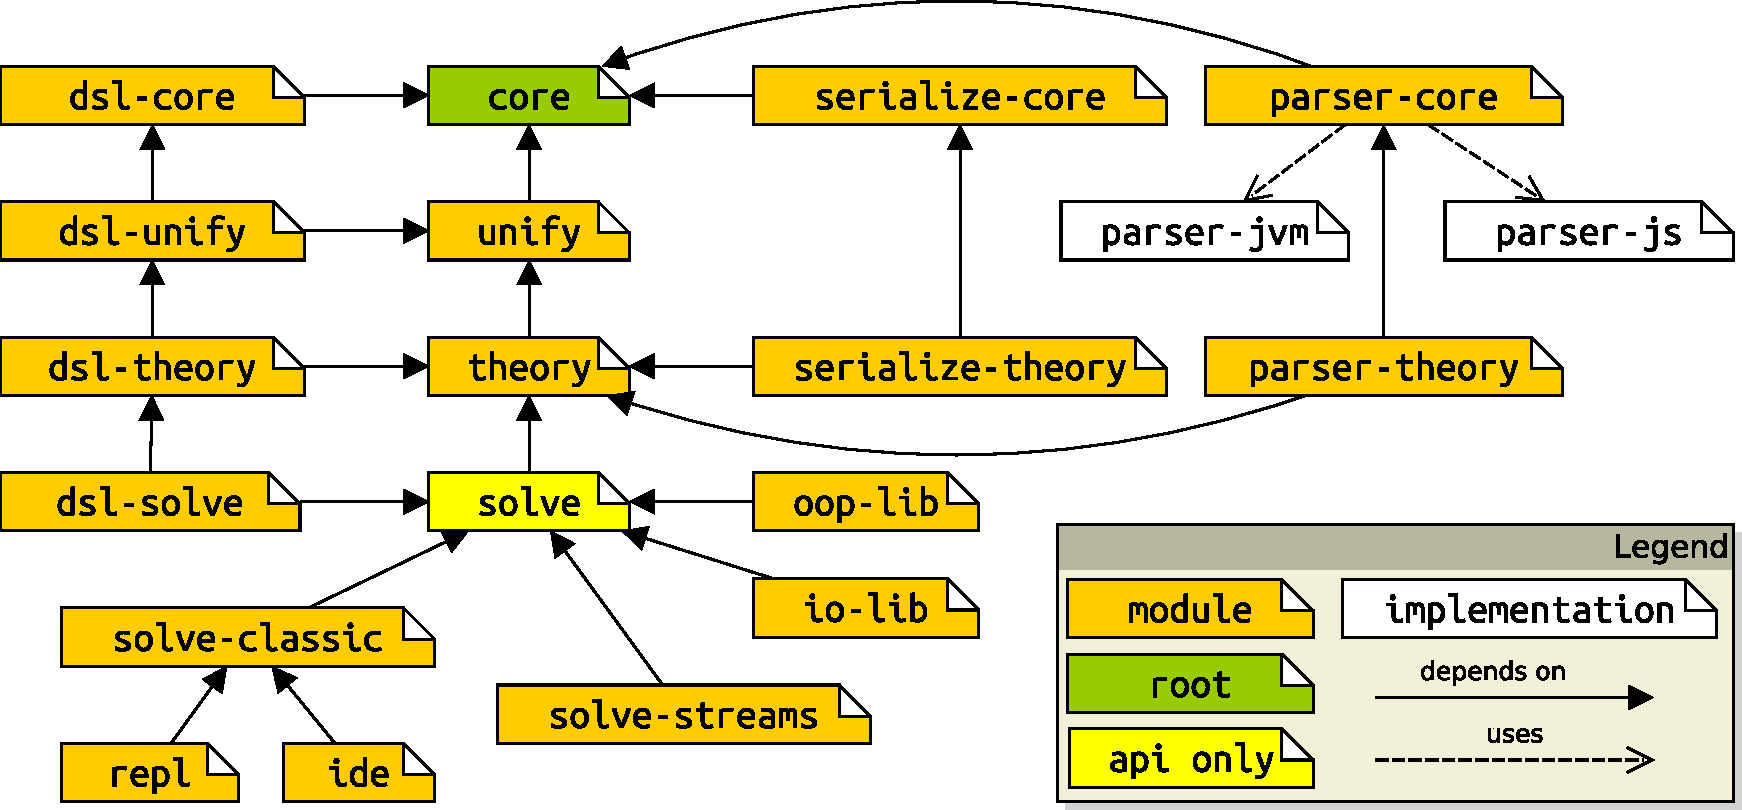
\includegraphics[width=\linewidth]{img/project-map.pdf}
    \end{center}

    \framebreak

    \begin{description}
        \item[\module{core}] provides \alert{knowledge representations} facilities \& common features
        %
        \begin{itemize}\small
            \item[eg] terms, clauses, substitutions, operators, term formatting, basic exceptions, etc.
        \end{itemize}

        \medskip

        \item[\module{unify}] provides support for \alert{logic unification}
        %
        \begin{itemize}\small
            \item[eg] customisable notion of unificator based on \cite{MartelliMontanari1982}
        \end{itemize}

        \medskip

        \item[\module{theory}] provides support in-memory \alert{storage \& indexing} of clauses
        %
        \begin{itemize}\small
            \item[eg] mutable/immutable and ordered/unordered \alert{collections of clauses} + \alert{logic theories}
        \end{itemize}
    
        \medskip
    
        \item[\module{solve}] provides generic support for \alert{resolution-related} stuff
        %
        \begin{itemize}\small
            \item[!] agnostic w.r.t. inference procedures \& resolution strategy 
            \item[eg] solvers, solutions, libraries, errors, flags, channels, etc.
        \end{itemize}

        \framebreak
    
        \item[\module{solve-*}] provide specific implementation for inference procedures \& \alert{resolution} strategy 
        %
        \begin{description}\small
            \item[\module{solve-classic}] SLD NF (Prolog-like) resolution \cite{Robinson65SLD,Clark77} based on Piancastelli's state machine \cite{tuprolog-sac08} (\alert{Prolog ISO \cite{prologISO-pt1} Compliant})
            \item[\module{solve-streams}] SLD NF (Prolog-like) resolution \cite{Robinson65SLD,Clark77} based on Enrico Siboni's master thesis and on \cite{Carlsson84}
        \end{description}

        \medskip

        \item[\module{parser-*}] supports \alert{parsing} of terms and clauses in Prolog syntax
        %
        \begin{description}\small
            \item[\module{parser-core}] supports parsing terms
            \item[\module{parser-theory}] supports parsing knowledge bases and streams of clauses 
            \item[\module{parser-jvm/js}] platform-specific implementations, based on ANTLR \cite{Parr2013} \hint{(not to be used directly!)}
        \end{description}

        \framebreak

        \item[\module{serialization-*}] support \alert{(de)serialization} of terms, clauses, knowledge bases in \alert{YAML/JSON}
        %
        \begin{description}\small
            \item[\module{serialization-core}] (de)serialization of terms and clauses
            \item[\module{serialization-theory}] (de)serialization of knowledge bases and theories
        \end{description}      
        
        \medskip

        \item[\module{dsl-*}] incrementally support the Kotlin-based DSL for LP described in~\cite{kotlinDSl4PrologWoa2020}, aimed at blending LP, FP, and OOP
        %
        \begin{description}\small
            \item[\module{dsl-core}] basic DSL for building terms/clauses in Kotlin
            \item[\module{dsl-unify}] extension of the DSL incuding \module{unify} facilities
            \item[\module{dsl-theory}] extension of the DSL incuding \module{theory} facilities
            \item[\module{dsl-solve}] extension of the DSL incuding \module{solve} facilities
        \end{description}   

        \framebreak

        \item[\module{repl}] command-line interface for Prolog
        
        \medskip

        \item[\module{ide}] JavaFX-based GUI for Prolog (customisable)
        
        \medskip

        \item[\module{io-lib}] Prolog ISO compliant Prolog library for I/O
        
        \medskip

        \item[\module{oop-lib}] Prolog library for OOP interoperability
        %
        \begin{itemize}\small
            \item essentially, lets Kotlin's and Java's OOP facilities be exploited from LP
            \item only JVM is currently supported, due to limitations in Kotlin's reflection API
        \end{itemize} 

    \end{description}
\end{frame}

\section{Knowledge Representation: the \module{core} Module}

\begin{frame}[allowframebreaks]{Main Abstractions from the \module{core} Module}
    \begin{block}{Terms and Clauses}\center\itshape\small
        Immutable data structures for terms and clauses in-memory representation \& manipulation
    \end{block}

    \begin{block}{Substitutions}\center\itshape\small
        Immutable data structures representing variables assignments, applicable to terms/clauses
    \end{block}

    \begin{block}{Operators and Operators Sets}\center\itshape\small
        Immutable data strucuters for representing logic operators and their esembles
    \end{block}

    \framebreak

    \begin{block}{Formatters}\center\itshape\small
        Functional objects aimed at converting terms/clauses into strings of customisable format
    \end{block}

    \begin{block}{Visitors}\center\itshape\small
        Functional objects aimed at easing type-dependent algorithms writing
    \end{block}   
    
    \begin{block}{Exceptions}\center\itshape\small
        Base exception types extensively exploited in all whole \twopkt{} project
    \end{block} 
\end{frame}

\subsection{The \kt{Term} Hierarchy}

\subsubsection{Main Sorts of \kt{Term}s and \kt{Clause}s}

\begin{frame}[allowframebreaks]{Term Hierarchy}
    \begin{center}
        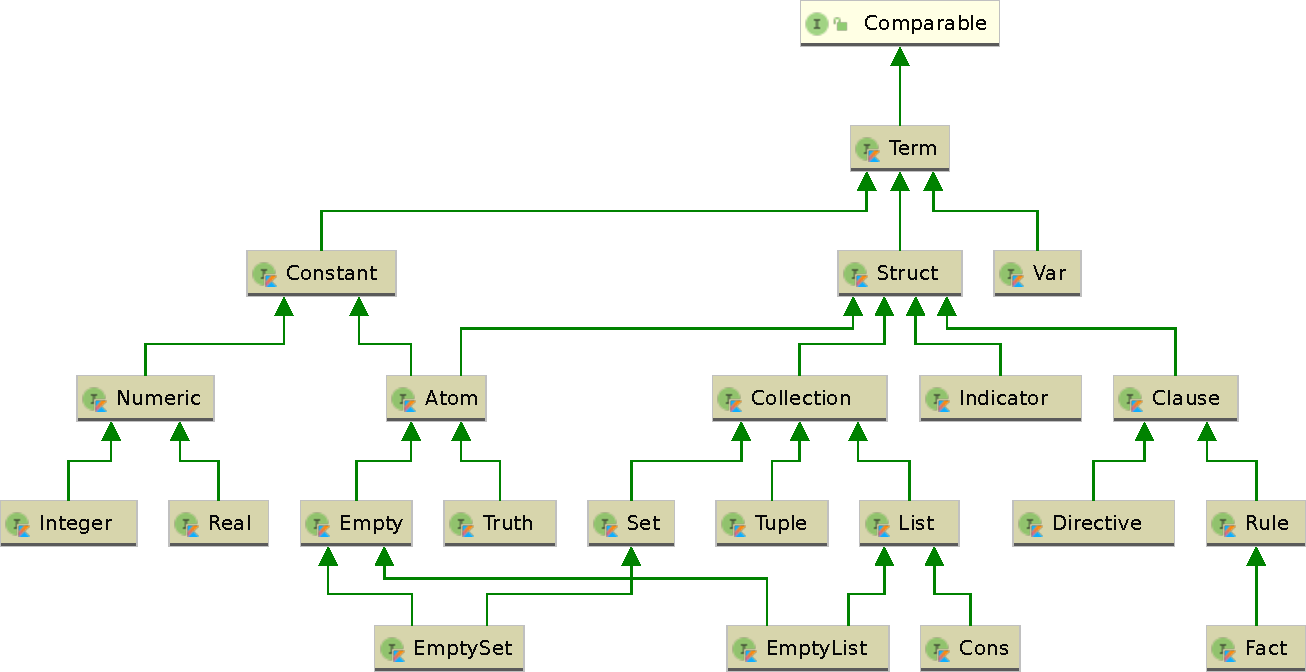
\includegraphics[width=\linewidth]{img/TermHierachy.pdf}
    \end{center}

    \begin{block}{Common Conventions}
        \begin{itemize}
            \item Only intefaces are publicly available, no classes
            \item Immutable design: all terms are immutable data structures
            \item The hierarchy is a DAG, not a tree
            \item Terms are totally ordered, as the are \kt{Comparable} among each others
            \item We call ``term'' any object which (indirectly) implements \kt{Term}
            %
            \begin{itemize}
                \item[!] there including clauses, i.e. instances of \kt{Clause}
            \end{itemize}
        \end{itemize}
    \end{block}
\end{frame}

\begin{frame}[allowframebreaks]{Sorts of Terms}
    \begin{block}{The \kt{Term} type}\centering\itshape
        Base type for all terms
    \end{block}
    %
    Main methods and properties:
        %
       \begin{description}
           \item[\kt{is\meta{SubType}: Boolean}] 
           \item[\kt{as\meta{SubType}(): \meta{SubType}}]  
           \item[\kt{castTo\meta{SubType}(): \meta{SubType}}]
           \item[\kt{freshCopy(): Term}]
           \item[\kt{equals(Any?): Boolean}]
           \item[\kt{equals(Term, Boolean): Boolean}]
           \item[\kt{structurallyEquals(Any?): Boolean}]
           \item[\kt{accept<T>(TermVisitor<T>): T}]
           \item[\kt{compareTo(Term): Int}]
           \item[\kt{toString(): String}]
       \end{description}
\end{frame}

\subsubsection{Creating \kt{Term}s}

\subsubsection{About \kt{Term}s' Immutable Design}

\subsection{\kt{Var}iables and \kt{Scope}s}

\subsection{\kt{Subtitution}s as First Class Entities}

\subsubsection{Refreshing \kt{Term}s}

\subsection{\kt{Operator}s and \kt{OperatorSet}s}

\subsection{Pattern Matching over \kt{Term}s Types}

\subsection{Exceptions}

\section{Logic Unification: the \module{unify} Module}

\section{Storing and Indexing Clauses: the \module{theory} Module}

\section{Generic Logic Resolution: the \module{solve} Module}

\subsection{\kt{Solver}s and the \kt{Solution}s}

\subsection{The \kt{ExecutionContext}}

\subsubsection{About \kt{Solver}s' Knowledge Bases}

\subsubsection{Extending \kt{Solver}s via \kt{Librarie}s}

\subsubsection{Communicating with the extenal world via \kt{Channel}s}

\subsubsection{Configuring \kt{Solver}s via \kt{Flag}s}

\subsubsection{Other sorts of custom fields}

\section{Custom \kt{Primitives}s, \kt{Function}s, and \kt{Libraries}s}

\subsection{About \kt{PrimitiveWrappers} and \kt{SideEffect}s}

\subsection{Logic \kt{Function}s and Evaluators}

\subsection{Writing \kt{Library}}

\section{Prolog as a State Machine: the \module{solve-classic} Module}

\section{Reading and Writing Data: the \module{io-lib} Module}

\section{OOP and Prolog: the \module{oop-lib} Module}

\subsection{\kt{Ref}erences: \kt{TypeRef}erences and \kt{ObjectRef}}

\subsection{OOP to/frm LP Conversions}

\subsection{Logic Predicates and Operators for OOP}

\section{LP + OOP + FP in Kotlin: the \module{dsl-*} Modules}

\section{Parsing Logic Knowledge: the \module{parser-*} Modules}

\section{(De)Serialising Logic Knowledge: the \module{serialize-*} Modules}

\section{Using \twopkt}

\subsection{As a library, for developers}

\subsubsection{For Java Developers}

\subsubsection{For JavaScript Developers}

\subsection{As an application, for end users}

\subsubsection{Graphical User Interface: the \module{ide} Module}

\subsubsection{Command Line Interface: the \module{cli} Module}

\section*{}
\frame{\titlepage}

\section*{\bibname}

\setbeamertemplate{page number in head/foot}{}

\begin{frame}[t,allowframebreaks,noframenumbering]\frametitle{\refname}
% \begin{frame}[c]\frametitle{\refname}
    \footnotesize
%    \scriptsize
    \bibliographystyle{plain}
    \bibliography{2p-kt-talk}
\end{frame}

%%%%%%%%%%%%%%%%%%%%%%%%%%%%%%%%%%%%%%%%%%%%%%%%%%%%%%%%%%%%%%%%%%%%%%%%%%%%%%%%
\end{document}
%%%%%%%%%%%%%%%%%%%%%%%%%%%%%%%%%%%%%%%%%%%%%%%%%%%%%%%%%%%%%%%%%%%%%%%%%%%%%%%%
